\chapter{Modeling of a vertical channel}\label{chapter:validation}

 This chapter presents the modelling of a vertical channel. Although the main interest of this master thesis work is about the circulating channel, we currently have very few experiments available for this kind of setup. Therefore, we first model the vertical channel to reproduce the simulation results from \cite{Wedin2001, Schillings2015}, and the experiment results from \cite{Boissonneau2000} to prove the validity of the numerical model adopted in this study. Afterward, we apply the same model to the circulating channel to get information currently not available in experiments. First, we will introduce the model assumptions and model setups. Afterward, we will present the mesh dependence study. Finally, the simulation results will be compared with the experimental data from Boissonneau et al. \cite{Boissonneau2000}, and the simulation results from Wedin et al.\cite{Wedin2001} to show the validity of the model. 

\section{Model assumptions}

\begin{enumerate}
    \item The fluid is incompressible and Newtonian.
    \item The flow field is assumed to be 2D.
    \item The flow field is assumed to isothermal.
    \item Bubble size is assumed to be constant and can be treated as solid particles.
    \item Bubble coalescence and breakup are neglected.
\end{enumerate}


\section{Vertical channel with forced flow}


\subsection{Geometry}

To reproduce the results from \cite{Boissonneau2000, Wedin2001}, we adopt the same geometry with \cite{Boissonneau2000}:

\begin{figure}[H]
    \centering
    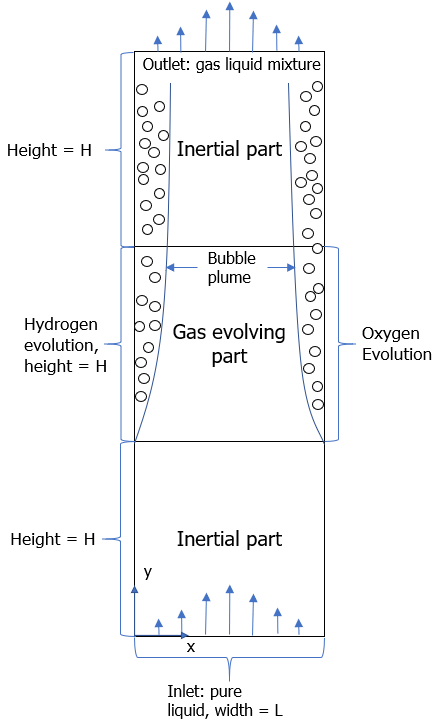
\includegraphics[scale=0.8]{sketchsquarechannel.png}
    \caption{A sketch for the vertical channel with forced flow, the channel is split into three parts in the vertical direction, where the middle part is the gas-evolving part, and the rest are the inertial part}
    \label{vertical}
\end{figure}

Where the channel width $L = 3 \, \mathrm{mm}$,and channel height $3H = 120  \, \mathrm{mm}$. Only in the middle part of the channel gas is evolved, the rest of the channel is called the inertial part. In the gas-evolving part, the gas is generated along the two electrodes, which are the two vertical boundaries on two different sides of the channel, resulting in two bubble plumes created. 

\subsection{Slip models}

The model adopted in this study is the bubbly flow model discussed in section \ref{section:bubblyflowmodel}.

% \begin{equation}
%          \rho_c \frac{\partial (\alpha_c\mathbf{u_c})}{\partial t}  
%         +  \rho_c \nabla \cdot (\alpha _c \mathbf{u_c u_c})  + \nabla \cdot (\alpha_c \mathbf{τ}) + \nabla p
%         = 0  \tag{\ref{eq:bubbly1}}
% \end{equation}

% \begin{equation}
%     \mathbf{τ} = -\mu (\nabla \mathbf{u_c} + \nabla \mathbf{u_c}^T-\frac{2}{3}(\nabla \cdot \mathbf{u_c})\mathbf{I})  \tag{\ref{eq:bubbly2}}
% \end{equation}

% \begin{equation}
%     \nabla \cdot (\alpha_d \mathbf{u_d} + \alpha_c \mathbf{u_c}) = 0 \tag{\ref{eq:bubbly3}}
% \end{equation}

% \begin{equation}
%     \frac{\partial \alpha_c}{ \partial t} + \nabla \cdot (\alpha_c \mathbf{u_c}) = 0 \tag{\ref{eq:bubbly4}}
% \end{equation}


% \begin{equation}
%     \mu = \frac{\mu_c}{1-\alpha_d} \tag{\ref{eq:bubbly5}}
% \end{equation}


The slip model adopted in this study is a combination of several elements discussed in section \ref{bubblebehavior} originally used by Wedin\cite{Wedin2001}:

\begin{equation}\label{eq:slipmodel}
    \mathbf{u_{slip}} = f(\mathbf{u_{Stokes}}+\mathbf{u_{Saff}}+\mathbf{u_{diffusion}})
\end{equation}

Where $f$ is the hindrance function in equation \ref{eq:richardson}, and the viscosity is always based on the viscosity model from equation \ref{eq:bubbly5}


\subsection{Material properties}

The solution in the flow channel is assumed to be $\mathrm{ Na_2SO_4 }$ with a $50 \, \mathrm{g/L}$ concentration (consistent with the experiment done by Boissonneau et al.\cite{Boissonneau2000}, which will be given as a comparison later in this section), while the bubble is a mixture of hydrogen and oxygen. Their material properties are given as below:


\begin{table}[h!]
\centering
\caption{Material propeties}
\label{materialpropeties}
\begin{tabular}{l l l l| l l l l}
\hline
    $\mu_c$  & liquid viscosity & $2 \times 10^{-3}$ & $\mathrm{ Pa \cdot s }$  &  $\rho_c$ & liquid density & $1.3 \times 10^{3}$ & $\mathrm{ kg/m^3 }$ \\

    $p$  & operating pressure & $1 \times 10^5$  & $\mathrm{ Pa }$ & $T$ & operating temperature& $300$ & $\mathrm{ \mathrm{K} }$\\
    
    $D_e$ & bubble diameter & $8 \times 10^{-5}$ & $\mathrm{ m }$ \\
    
\hline
\end{tabular}
\end{table}


\subsection{Boundary conditions}

As shown in figure \ref{vertical}, pure liquid flows into the channel,  so at the bottom, the boundary condition is given as:

\begin{equation}
    u_{cy}(y=0) = 0.06 \, \mathrm{m/s}     
\end{equation}

\begin{equation}
    u_{cx}(y=0) = 0 \, \mathrm{ m/s }
\end{equation}

\begin{equation}
    \mathbf{u_d}(y=0) = 0 \, \mathrm{ m/s }
\end{equation}

At two sides of the channel, the boundary condition for the liquid phase is no-slip, for the gas phase is inlet at the gas evolving part and no-slip at the inertial part.


\begin{equation}
    \mathbf{u_{c}}(x = 0) = 0 \, \mathrm{ m/s }
\end{equation}

\begin{equation}
    \mathbf{u_{c}}(x = L) = 0 \, \mathrm{ m/s }
\end{equation}

\begin{equation}
    \mathbf{u_{d}}(x = 0) = 0 \, \mathrm{ m/s }, \quad for  \quad 0 \leq y \leq H \quad and \quad 2H \leq y \leq 3H
\end{equation}

\begin{equation}
    \mathbf{u_{d}}(x = L) = 0 \, \mathrm{ m/s }, \quad for  \quad 0 \leq y \leq H \quad and \quad 2H \leq y \leq 3H
\end{equation}


As discussed in the previous chapter, one of the challenges is that the lack of information about the volume fraction at the wall region hinders the comprehensive modelling of the gas evolution process. In the bubbly flow model adopted in this work, the gas is treated as an injection, and we only need information about the gas flux, which lumps the volume fraction and gas intrinsic velocity into one variable based on equation \ref{eq:gasevolution}:
\begin{equation}\label{eq:hydrogenevolution}
    N_{H_2}(x = 0) = \alpha_d u_{dx} = \frac{RTi_{av}}{2pF}, \quad for  \quad H \leq y \leq 2H
\end{equation}

\begin{equation}\label{eq:oxygenevolution}
    N_{O_2}(x = L) = \alpha_d u_{dx} = -\frac{RTi_{av}}{4pF}, \quad for  \quad H \leq y \leq 2H
\end{equation}

At the top of the channel, the velocity boundary condition is treated as a pressure outlet, which is essentially a zero gradient boundary. To close the model, we also need a Dirichlet boundary condition for pressure; the pressure is fixed to zero at the top surface with hydrostatic pressure distribution in the channel as the initial condition.

\subsection{Meshing}

Given the rectangular shape of the vertical channel, structured mesh with quadrilateral elements is used:

\begin{figure}[H]
    \centering
    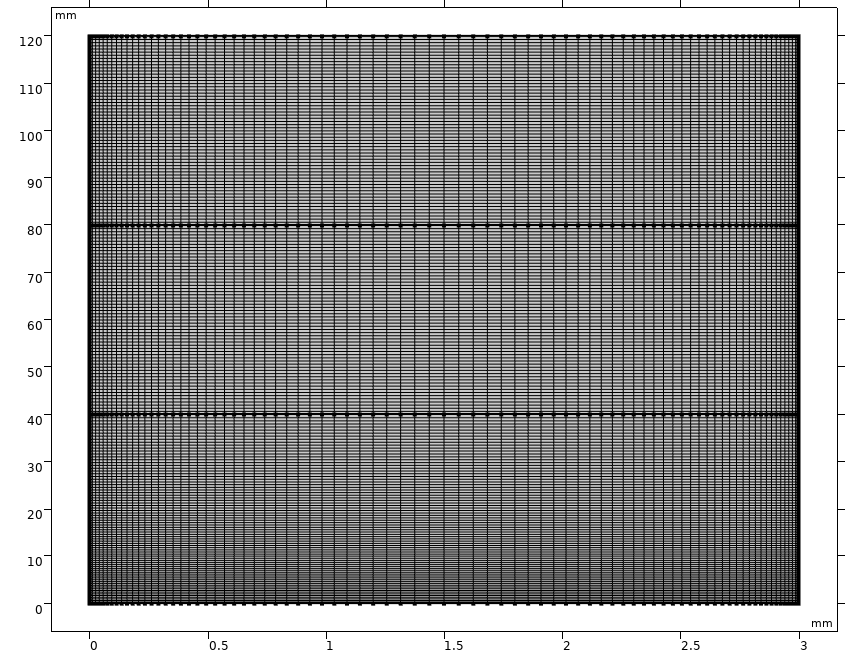
\includegraphics[width = \textwidth]{mesh.png}
    \caption{The mesh used to study the vertical channel flow, horizontal $\times$ vertical element number $ =  80  \times 200 $.}
    \label{mesh}
\end{figure}

As shown in figure \ref{mesh}, the mesh is finer at the liquid inlet at the bottom, and the gas inlet at the left and right side of the channel, coarser at the rest of the domain, so that we can keep a balance between accuracy and computation cost.

\subsection{Mesh dependence study}

To make sure that the mesh is fine enough for the problem studied, we need to compare the results obtained with different mesh. In this study, three structured mesh with quadrilateral elements at different levels of refinement is used; they are respectively $40 \times 350$, $60 \times 450$, and $80 \times 600$. The first one is shown in the previous part. The other two mesh is similar, only that the mesh is not refined at the bottom inlet boundary anymore.

The comparison between these three meshes is shown in figure \ref{meshstudy}. From the figure, we can see that results obtained with three kinds of mesh are nearly the same; thus, we can choose to use the coarser mesh, which reaches convergence faster.

\begin{figure}[H]
    \centering
    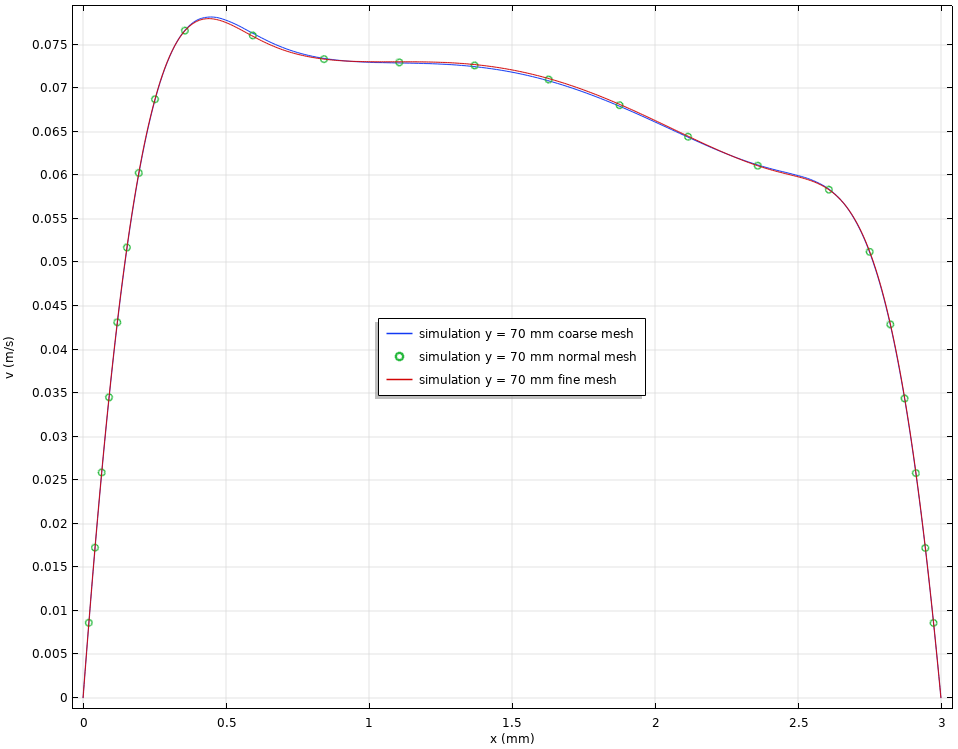
\includegraphics[width=1\textwidth]{meshstudy.png}
    \caption{Mesh dependence study, the results are chosen at $y = 70 \, \mathrm{ mm }$. Coarse mesh: $40 \times 350$, normal mesh: $60 \times 450$, fine mesh: $80 \times 600$}
    \label{meshstudy}
\end{figure}

\subsection{Velocity profile comparison}

The experimental data used here comes from Boissonneau et al. \cite{Boissonneau2000}, while the simulation data is based on the mesh in figure \ref{meshstudy} (40 $ \times$ 350), the comparison shown in figure \ref{squarechannelresult}. From the figure, we can see that before the gas evolving part, the profile is Poiseuille flow, while after entering the gas evolving part, the velocity at the near-wall region is lifted by the bubbles. The overall behaviour matches with the experiment, while it seems that from the experiment, the lifting effect from oxygen bubbles are more significant than the predicted results. The reason could be that that oxygen bubbles tend to have a larger diameter, which means larger buoyancy force, while in the simulation we can only use one fixed bubble diameter for the modelling of both hydrogen and oxygen bubbles. 

\begin{figure}[H]
\centering
\begin{subfigure}{0.5\textwidth}
  \centering
  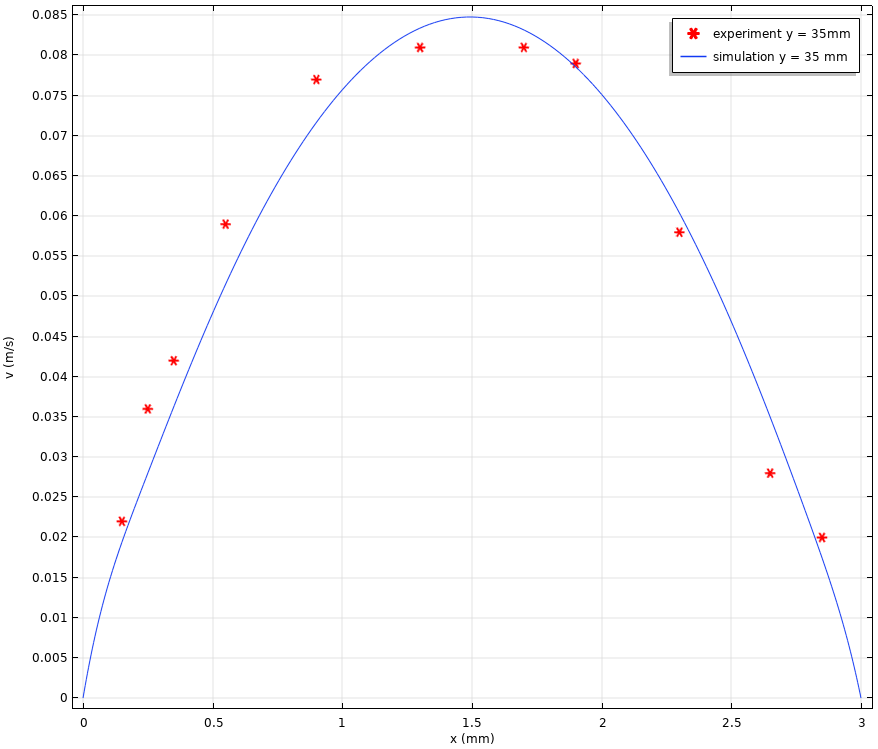
\includegraphics[width=1\linewidth]{squarechannelvalidation.png}
  \caption{liquid velocity profile at y direction at $ y = 35 \, \mathrm{mm} $}
  \label{triangular}
\end{subfigure}%
\begin{subfigure}{0.5\textwidth}
  \centering
  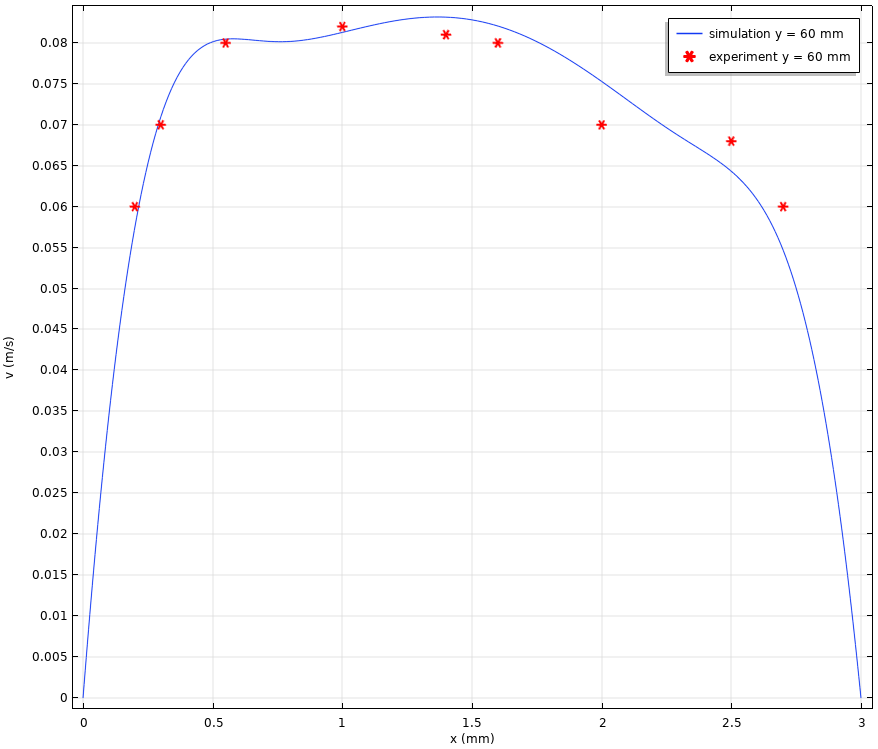
\includegraphics[width=1\linewidth]{squarechannelvalidation1.png}
  \caption{liquid velocity profile at y direction at $ y = 60 \, \mathrm{mm} $}
  \label{rectangular}
\end{subfigure}
\begin{subfigure}{0.5\textwidth}
  \centering
  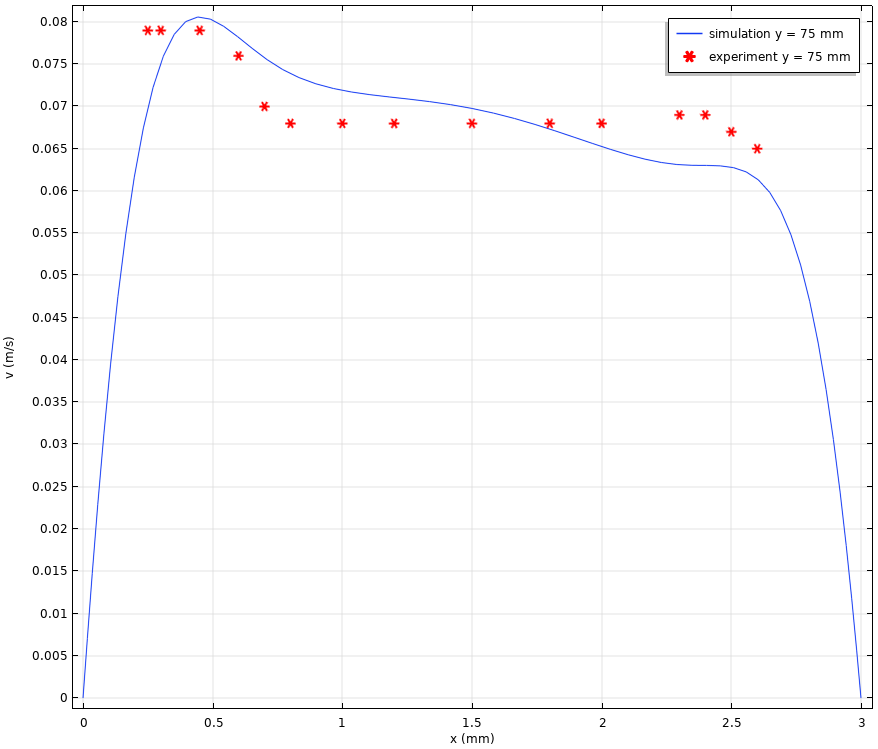
\includegraphics[width=1\linewidth]{squarechannelvalidation2.png}
  \caption{liquid velocity profile at y direction at $ y = 75 \, \mathrm{mm} $}
  \label{rectangular}
\end{subfigure}
\caption{Liquid velocity profile at y direction across the channel at different heights in the channel, experimental data comes from Boissonneau et al.\cite{Boissonneau2000}, $i_{av} = 1000 \, \mathrm{A/m^2}$, In (b) and (c) we can see the velocity at the near wall region becomes significantly higher, which is driven by the bubbles}
\label{squarechannelresult}
\end{figure}


\subsection{Volume fraction profile comparison}

From the experimental data provided by Boissonneau et al. \cite{Boissonneau2000}, we could only compare the velocity profile. Regarding the volume fraction profile, however, there are many discrepancies among literature even when under similar operating conditions \cite{abdelouahed2014hydrodynamics, Mat2005, philippe2005modelling}. Since the bubbly model used in this study is based on the one originally proposed by Wedin et al.\cite{Wedin2001}, here we also give a comparison between the results in this study and the results from Wedin. The results from Wedin also include gas evolution from the left side, so we also set equation \ref{eq:oxygenevolution} to 0, the comparison is shown in figure \ref{volumefractioncomparison}.

From the volume fraction comparison in figure \ref{volumefractioncomparison} we can see the simulation done in this study nicely reproduced the results from the original model proposed by Wedin et al. However, it does not mean that this volume fraction profile accurately predicted the one in reality. As stated before, there are many discrepancies among literature concerning volume fraction profile even when under similar conditions \cite{abdelouahed2014hydrodynamics, Mat2005, philippe2005modelling}. In this study, we aim to analyze the role of different forces, e.g.: dispersion force, lift force, diffusion, etc. through the study of the model proposed by Wedin et al., since their model provides more potential elements that could impact the volume fraction profiles, and thus controlling the plume thickness and velocity throughout the channel.

\begin{figure}
\centering
\begin{subfigure}{1\textwidth}
  \centering
  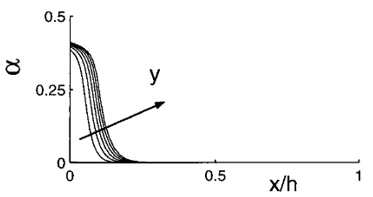
\includegraphics[width=1\linewidth]{Wedinvolumeprofile.png}
  \caption{volume fraction profile from Wedin et al. \cite{Wedin2001} at different height}
  \label{Wedinprofile}
\end{subfigure}%

\begin{subfigure}{1\textwidth}
  \centering
  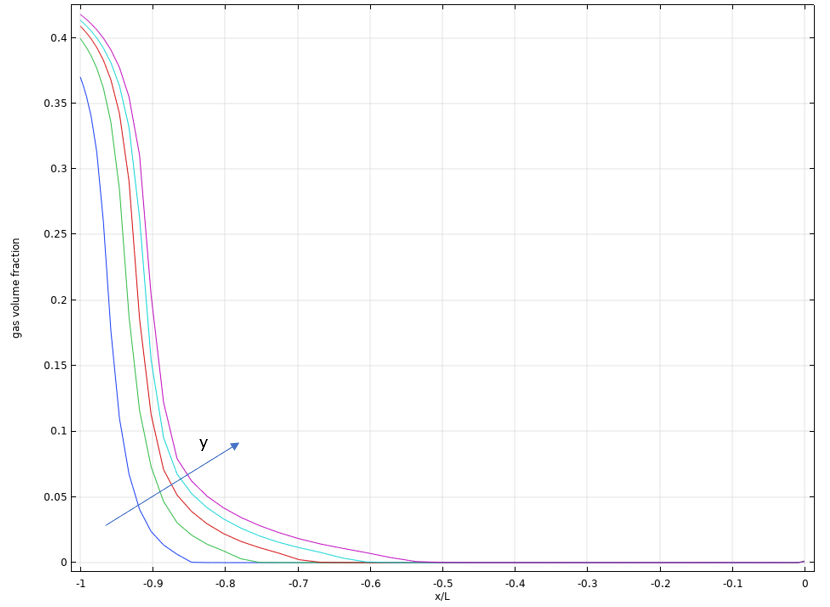
\includegraphics[width=1\linewidth]{myvolumeprofile.png}
  \caption{volume fraction profile from this study at different height}
  \label{myprofile}
\end{subfigure}
\caption{Volume fraction profile comparison, (a) is the simulation results from \cite{Wedin2001}, (b) is the simulation results in this work, $i_{av} = 2000 \,  \mathrm{A/m^2}$, $L =  1 \, \mathrm{cm}$. We can see the overall profile matches well}
\label{volumefractioncomparison}
\end{figure}

